\documentclass[../../szobeli.tex]{subfiles}

\begin{document}

\begin{center}
    \noindent\fbox{%
    	\parbox{160mm}{
			\underline{\textbf{Élhozzáadási lemma}} erdő, \textbf{fa}, fák egyszerűbb tulajdonságai: \underline{két levél}, \underline{erdők élszáma}. \textbf{Feszítőfa} \underline{létezése}, feszítőfához tartozó alapkörök és alap vágások.
        }
    }
\end{center}
    \begin{itemize}
        \item \underline{\textbf{Élhozzáadási lemma (ÉHL):}} Legyen $G$ irányítatlan gráf és $G' = G + e$. Ekkor az alábbi két esetből pontosan egy valósul meg. 
            \begin{itemize} 
                \item[(1)] $G$ és $G'$ komponensei megegyeznek, de $G'$-nek eggyel több köre van, mint $G$-nek.
                \item[(2)] $G$ és $G'$ körei megegyeznek, de $G'$-nek eggyel kevesebb komponense van, mint $G$-nek. 
            \end{itemize}
        \item Erdő: A körmentes irányítatlan gráfot \textcolor{red}{erdőnek} nevezzük. 
        \item \textbf{Fa:} Az összefüggő, körmentes irányítatlan gráf neve \textcolor{red}{fa}. 
            \begin{itemize}
                \item $G$ erdő $\Longleftrightarrow  G$ minden komponense fa.
                \item $G$ $n$-csúcsú, $k$-komponensű erdő $\Rightarrow |E(G)| = n-k$.
                \item \textbf{Biz:} Építsük fel $G$-t a $\overline{K_n}$ üresgráfból az élek egyenkénti behúzásával. $G$ körmentes, ezért az ÉHL miatt minden él zöld: behúzásakor 1-gyel csökken a komponensek száma. A $\overline{K_n}$ üresgráfnak $n$ komponense van, $G$-nek pedig $k$. Ezért pontosan $n-k$ zöld élt kellett behúzni $G$ felépítéséhez.
            \end{itemize}
        \item \underline{Két levél:} Legyen $F$ egy tetszőleges fa $n$ csúcson. Ekkor ha $n \geq 2$, akkor $F$-nek legalább két levele van.
            \begin{itemize}
                \item \textbf{Biz:} (Algebrai út) A KFL miatt $\sum_{v\in V(G)}(d(v)-2)=\sum_{v\in V(G)}d(v)-2n=2(n-1)-2n=-2$. $F$ minden $v$ csúcsára $d(v) \geq 1$ teljesül, ezért $d(v) - 2 \geq -1$. A fenti összeg csak úgy lehet $-2$, ha $F$-nek legalább 2 levele van.
                \item \textbf{Biz:} (Kombinatorikus út) Induljunk el $F$ egy tetszőleges $v$ csúcsából egy sétán, és haladjunk, amíg tununk. Ha sosem akadunk el, akkor előbb-utóbb ismétlődik egy csúcs, és kört találunk. Ezért elakadunk, és az csakis egy $v$-től különböző $u$ levélben történhet. Ha $d(v)=1$, akkor $v$ egy $u$-tól különböző levél. Ha $d(v) \geq 2$, akkor sétát indíthatunk $v$-ből egy másik él mentén. Ekkor egy $u$-tól különböző levélben akadunk el.
            \end{itemize}
        \item \textbf{Feszítőfa} 
        
            $F$ a $G$ gráf feszítőfája (ffa), ha $F$ egy $G$-ből éltörésekkel kapható fa. Ha $G$-nek van feszítőfája $\Leftrightarrow$ (akkor) összefüggő.
            
            Építsük fel a $G$ gráfot az élek egymás utái behúzásával, és az ÉHL szerinti kiszínezésével!
            
            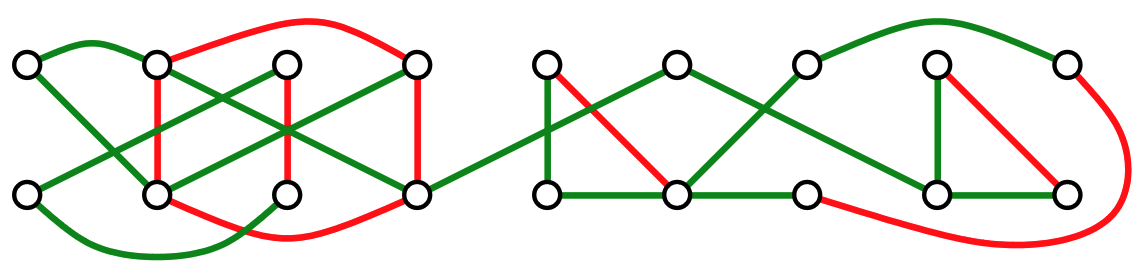
\includegraphics[scale=0.4]{./img/1.png}
            
            Legyen \textcolor{green}{$G'$} a $G$ gráf piros élei törlésével keletkező feszítő részgráf! \textcolor{green}{$G'$} biztosan körmentes lesz, hiszen a zöld élek sosem alkottak kört a korábbi élekkel. \textcolor{green}{$G'$} minden \textcolor{green}{$K'$} komponense részhalmaza $G$ egy $K$ komponensének. Ha $K' \neq K$, akkor $G$-nek van olyan éle, ami kilép $K'$-ből. Ezen élek mind pirosak \textcolor{green}{$K'$} definíciója miatt. Legyen $e$ ezek közül az elsőnek kiszínezett. Az $e$ él nem tudott kört alkotni a korábbn kiszínezettekel, így nem lehet piros: ellentmondás. Ezek szerint $G$ egy \textcolor{green}{$G'$} komponensei megegyeznek.

            \textcolor{orange}{\textbf{Köv:}} A $G$ gráf zöld élei olyan \textcolor{green}{$G'$} feszítő részgráfot alkotnak, ami erdő, és komponensei megegyeznek $G$ komponenseivel. 

            \textcolor{blue}{\textbf{Def:}} $F$ a $G$ gráf \textcolor{red}{feszítőfája} (\textcolor{red}{ffája}), ha $F$ egy $G$-ből éltörlésekkel kapható fa.

            \textcolor{orange}{\textbf{Állítás:}} ($G$-nek van feszítőfája) $\Longleftrightarrow$ ($G$ összefüggő)

            \textcolor{green}{\textbf{Biz:}} $\Rightarrow$: Legyen $F$ a $G$ feszítőfája. $F$ összefüggő, és $V(F)=V(G)$, tehát $G$ bármely két csúcsa között vezet $F$-beli út.

            $\Leftarrow$: Építsük fel $G$-t az álek egyenkénti behúzásával és kiszínezésével. Láttuk, hogy a zöld élek egy \textcolor{green}{$F$} erdőt alkotnak, aminek egyetlen komponense van, hiszen $G$ is egy komponensű. Ezek szerint \textcolor{green}{$F$} olyan fa, ami $G$-ből éltörlésekkel kapható. 

            \textcolor{blue}{\textbf{Megj:}} Ha egy nem feltétlenül összefüggő $G$ gráf éleit a fenti módon kiszínezzük, akkor a zöld élek $G$ minden komponensének egy \textcolor{green}{$F$} feszítőfáját alkotják. Nem összefüggő $G$ esetén a zöld élek alkotta feszítő részgráf neve a $G$ \textcolor{red}{feszítő erdeje}.

        \item Alapvágás, alapkör: 
        
            A $G$ gráf $F$ feszítőfájának $f$ éléhez tartozó \textcolor{red}{alap vágást} $G$ azon élei alkotják, amik az $F-f$ által létrehozott két komponens között futnak. 
            
            Az $e \in E(G) \backslash E(F)$ éléhez tarozó \textcolor{red}{alapkör} pedig az $F+e$ köre.  
            
            \textbf{Megf:} Tfh $f \in F$ és $e \in E(G) \backslash E(F)$. Ekkor ($F-f+e$ ffa) $\Longleftrightarrow$ ($f$ benne van $e$ alapkörében) $\Longleftrightarrow$ ($e$ benne van $f$ alap vágásában).
    \end{itemize}

\end{document}